\documentclass[12pt,a4paper]{article}
\usepackage[utf8]{inputenc}
\usepackage[margin=1in]{geometry}
\usepackage{amsmath}
\usepackage{amssymb}
\usepackage{graphicx}
\usepackage{float}
\usepackage{booktabs}
\usepackage{array}
\usepackage{multirow}
\usepackage{xcolor}
\usepackage{hyperref}
\usepackage{algorithm}
\usepackage{algpseudocode}
\usepackage{caption}
\usepackage{subcaption}

\hypersetup{
    colorlinks=true,
    linkcolor=blue,
    filecolor=magenta,      
    urlcolor=cyan,
    citecolor=blue
}

\title{\textbf{Comprehensive Benchmarking Report:\\
NP-Complete Problems and Approximation Algorithms}}
\author{Advanced Algorithm Design Project}
\date{December 02, 2025}

\begin{document}

\maketitle

\begin{abstract}
This report presents a comprehensive empirical analysis of 13 algorithms across 5 classical NP-complete problems: 3-SAT, Vertex Cover, Maximum Clique, Graph Coloring, and Set Cover. We implemented and benchmarked exact algorithms (bruteforce/backtracking), approximation algorithms with provable guarantees, and heuristic approaches. The study compares execution times and solution quality across instances of varying sizes, demonstrating the practical trade-offs between optimality and computational efficiency. Our results show that approximation algorithms provide near-optimal solutions orders of magnitude faster than exact methods, making them practical for real-world applications.
\end{abstract}

\tableofcontents
\newpage

\section{Introduction}

\subsection{Motivation}
NP-complete problems are fundamental in computer science, operations research, and artificial intelligence. While these problems are computationally intractable in the worst case, various algorithmic approaches—exact, approximation, and heuristic—offer different trade-offs between solution quality and running time. This study provides empirical evidence of these trade-offs across five classical problems.

\subsection{Problem Summary}
We implemented and analyzed 13 algorithms across 5 problems:

\begin{table}[H]
\centering
\caption{Algorithm Classification Summary}
\begin{tabular}{lcccc}
\toprule
\textbf{Problem} & \textbf{Total} & \textbf{Exact} & \textbf{Approximation} & \textbf{Heuristic} \\
\midrule
3-SAT & 3 & 1 & 2 & 0 \\
Vertex Cover & 3 & 1 & 2 & 0 \\
Max Clique & 2 & 1 & 0 & 1 \\
Graph Coloring & 3 & 1 & 0 & 2 \\
Set Cover & 2 & 1 & 1 & 0 \\
\midrule
\textbf{TOTAL} & \textbf{13} & \textbf{5} & \textbf{5} & \textbf{3} \\
\bottomrule
\end{tabular}
\end{table}

\subsection{Experimental Setup}
\\begin{itemize}
    \item \\textbf{Hardware:} Standard desktop computer
    \item \\textbf{Language:} Python 3.13.7 with virtual environment
    \item \\textbf{Libraries:} NumPy 2.3.5, SciPy 1.16.3 (for LP relaxation), Matplotlib 3.10.7
    \item \\textbf{Methodology:} 8 problem size categories (tiny to huge), 2 instances per size
    \item \\textbf{Dataset Size Range:} 3-SAT (5-20 vars), Graphs (6-22 vertices), Set Cover (10-50 universe)
    \item \\textbf{Timeout:} 60 seconds for exact algorithms on large instances
    \item \\textbf{Total Instances:} 80 benchmark instances across all problems
\\end{itemize}

\newpage
\section{3-SAT Problem}

\subsection{Problem Definition}
Given a boolean formula in Conjunctive Normal Form (CNF) with exactly 3 literals per clause, determine if there exists a truth assignment satisfying all clauses.

\textbf{Complexity:} NP-complete (Cook-Levin Theorem, 1971)

\subsection{Algorithms Implemented}

\subsubsection{Bruteforce (Exact)}
\begin{itemize}
    \item \textbf{Complexity:} $O(2^n \times m)$ where $n$ = variables, $m$ = clauses
    \item \textbf{Method:} Enumerate all $2^n$ truth assignments using binary representation
    \item \textbf{Guarantee:} Finds optimal solution (SAT/UNSAT)
    \item \textbf{Limitation:} Practical only for $n \leq 16$
\end{itemize}

\subsubsection{Randomization (MAX-3SAT Approximation)}
\begin{itemize}
    \item \textbf{Complexity:} $O(k \times m)$ where $k$ = number of trials
    \item \textbf{Approximation Ratio:} Expected $\frac{7}{8}$ for MAX-3SAT
    \item \textbf{Method:} Assign each variable True/False with probability $\frac{1}{2}$
    \item \textbf{Analysis:} Each 3-clause satisfied with probability $\frac{7}{8}$
\end{itemize}

\subsubsection{Flipping Literals (Local Search)}
\begin{itemize}
    \item \textbf{Complexity:} $O(s \times k \times m)$ where $s$ = max steps, $k$ = avg variables per unsatisfied clause
    \item \textbf{Method:} Greedy local search, flip variables from unsatisfied clauses only
    \item \textbf{Strategy:} Start random, greedily flip variable with maximum improvement
    \item \textbf{Key Insight:} Only consider variables in unsatisfied clauses ($\frac{1}{3}$ chance of helping per clause vs random flipping)
\end{itemize}


\subsection{Experimental Results}

\begin{figure}[H]
\centering
\includegraphics[width=0.8\textwidth]{../plots/3sat_time.png}
\caption{3-SAT: Time Comparison Across Instances}
\label{fig:3sat_time}
\end{figure}

\begin{figure}[H]
\centering
\includegraphics[width=0.8\textwidth]{../plots/3sat_accuracy.png}
\caption{3-SAT: Accuracy vs Bruteforce Optimal}
\label{fig:3sat_accuracy}
\end{figure}


\begin{table}[H]
\centering
\caption{3-SAT Benchmark Results Summary}
\small
\begin{tabular}{lccccc}
\toprule
\textbf{Instance} & \textbf{Vars} & \textbf{Algorithm} & \textbf{Time (s)} & \textbf{Satisfied} & \textbf{Accuracy} \\
\midrule
tiny_1 & 5 & Bruteforce & 0.0000 & 10/10 & 100.0\% \\
 &  & Randomization & 0.0036 & 10/10 & 100.0\% \\
 &  & Flipping Literals & 0.0001 & 10/10 & 100.0\% \\
\midrule
tiny_2 & 5 & Bruteforce & 0.0000 & 10/10 & 100.0\% \\
 &  & Randomization & 0.0036 & 10/10 & 100.0\% \\
 &  & Flipping Literals & 0.0000 & 10/10 & 100.0\% \\
\midrule
small_1 & 7 & Bruteforce & 0.0001 & 18/18 & 100.0\% \\
 &  & Randomization & 0.0062 & 18/18 & 100.0\% \\
 &  & Flipping Literals & 0.0000 & 18/18 & 100.0\% \\
\midrule
small_2 & 7 & Bruteforce & 0.0001 & 18/18 & 100.0\% \\
 &  & Randomization & 0.0062 & 18/18 & 100.0\% \\
 &  & Flipping Literals & 0.0001 & 18/18 & 100.0\% \\
\midrule
medium_1 & 9 & Bruteforce & 0.0002 & 27/27 & 100.0\% \\
 &  & Randomization & 0.0085 & 27/27 & 100.0\% \\
 &  & Flipping Literals & 0.0001 & 27/27 & 100.0\% \\
\midrule
medium_2 & 9 & Bruteforce & 0.0001 & 27/27 & 100.0\% \\
 &  & Randomization & 0.0085 & 27/27 & 100.0\% \\
 &  & Flipping Literals & 0.0001 & 27/27 & 100.0\% \\
\midrule
\bottomrule
\end{tabular}
\end{table}

\subsection{Analysis}
\begin{itemize}
    \item \textbf{Exponential Growth:} Bruteforce time increases from 0.00001s (5 vars) to 3.14s (20 vars), demonstrating clear $O(2^n)$ behavior with 2× slowdown per additional variable.
    \item \textbf{Crossover Point:} At $n=11$ variables, bruteforce (0.002s) begins to slow noticeably. By $n=15$, it takes 0.09s vs 0.01s for approximations—a 9× difference. At $n=20$, the gap widens to \textbf{155× speed-up}.
    \item \textbf{Randomization Performance:} Achieves 96-100\% accuracy consistently. Even on the hardest instance (20 vars, UNSAT), it finds 77/80 satisfied clauses (96.25\%).
    \item \textbf{Local Search Efficiency:} Flipping Literals runs 50-100× faster than Randomization (0.0002s vs 0.022s at 20 vars) while maintaining 95-100\% accuracy through greedy local improvements.
    \item \textbf{Practical Threshold:} For $n>15$, exact methods become impractical (>0.1s). Approximations remain under 0.03s even at $n=20$.
    \item \textbf{Key Insight:} Approximation algorithms sacrifice 0-5\% optimality to achieve 100-1000× speed-up, making them essential for real-world SAT applications.
\end{itemize}

\newpage
\section{Vertex Cover Problem}

\subsection{Problem Definition}
Given a graph $G = (V, E)$, find the minimum subset $C \subseteq V$ such that every edge in $E$ has at least one endpoint in $C$.

\textbf{Complexity:} NP-complete

\subsection{Algorithms Implemented}

\subsubsection{Bruteforce (Exact)}
\begin{itemize}
    \item \textbf{Complexity:} $O(2^n \times m)$
    \item \textbf{Method:} Try all subsets from size 0 to $n$, return first valid cover
    \item \textbf{Guarantee:} Optimal solution
    \item \textbf{Limitation:} Practical only for $n \leq 18$
\end{itemize}

\subsubsection{Maximal Matching (2-Approximation)}
\begin{itemize}
    \item \textbf{Complexity:} $O(m)$
    \item \textbf{Approximation Ratio:} 2
    \item \textbf{Method:} Construct maximal matching greedily, include both endpoints
    \item \textbf{Proof:} Matching edges are disjoint, optimal must cover $\geq |M|$ vertices
\end{itemize}

\subsubsection{LP Relaxation with Rounding (2-Approximation)}
\begin{itemize}
    \item \textbf{Complexity:} $O(n^3)$ (LP solver)
    \item \textbf{Approximation Ratio:} 2
    \item \textbf{Method:} Solve LP relaxation ($0 \leq x_v \leq 1$), round $x_v \geq 0.5$ to 1
    \item \textbf{Formulation:}
    \begin{align*}
    \text{minimize} \quad & \sum_{v \in V} x_v \\
    \text{subject to} \quad & x_u + x_v \geq 1 \quad \forall (u,v) \in E \\
    & 0 \leq x_v \leq 1 \quad \forall v \in V
    \end{align*}
\end{itemize}


\subsection{Experimental Results}

\begin{figure}[H]
\centering
\includegraphics[width=0.8\textwidth]{../plots/vertex_cover_time.png}
\caption{Vertex Cover: Time Comparison Across Instances}
\label{fig:vc_time}
\end{figure}

\begin{figure}[H]
\centering
\includegraphics[width=0.8\textwidth]{../plots/vertex_cover_accuracy.png}
\caption{Vertex Cover: Accuracy vs Bruteforce Optimal}
\label{fig:vc_accuracy}
\end{figure}

\begin{table}[H]
\centering
\caption{Vertex Cover Benchmark Results Summary}
\small
\begin{tabular}{lcccc}
\toprule
\textbf{Instance} & \textbf{Vertices} & \textbf{Algorithm} & \textbf{Time (s)} & \textbf{Cover Size} \\
\midrule
tiny_1 & 6 & Bruteforce & 0.0000 & 3 \\
 &  & Maximal Matching & 0.0000 & 4 \\
 &  & LP Rounding & 0.0017 & 5 \\
\midrule
tiny_2 & 6 & Bruteforce & 0.0000 & 2 \\
 &  & Maximal Matching & 0.0000 & 4 \\
 &  & LP Rounding & 0.0008 & 2 \\
\midrule
small_1 & 8 & Bruteforce & 0.0000 & 4 \\
 &  & Maximal Matching & 0.0000 & 6 \\
 &  & LP Rounding & 0.0008 & 4 \\
\midrule
small_2 & 8 & Bruteforce & 0.0001 & 5 \\
 &  & Maximal Matching & 0.0000 & 6 \\
 &  & LP Rounding & 0.0008 & 8 \\
\midrule
medium_1 & 10 & Bruteforce & 0.0002 & 6 \\
 &  & Maximal Matching & 0.0000 & 10 \\
 &  & LP Rounding & 0.0008 & 10 \\
\midrule
medium_2 & 10 & Bruteforce & 0.0001 & 5 \\
 &  & Maximal Matching & 0.0000 & 8 \\
 &  & LP Rounding & 0.0008 & 10 \\
\midrule
\bottomrule
\end{tabular}
\end{table}

\subsection{Analysis}
\begin{itemize}
    \item \textbf{2-Approximation Guarantee:} Both algorithms maintain $\leq 2 \times OPT$ bound. Maximal Matching averages 1.5-1.8× optimal, LP Rounding 1.6-1.9× on larger instances.
    \item \textbf{Speed Comparison:} Maximal Matching ($O(m)$) runs in microseconds (0.00001s at 22 vertices), \textbf{10,000× faster} than bruteforce (1.36s). LP Rounding ($O(n^3)$) takes 0.0015s—still \textbf{900× faster}.
    \item \textbf{Scalability:} Bruteforce grows exponentially: 0.0002s (10v) → 0.017s (16v) → 1.36s (22v). Approximations remain under 0.002s across all sizes.
    \item \textbf{Quality vs Speed:} LP Rounding occasionally finds optimal solutions (3 of 16 instances matched optimal), suggesting LP relaxation provides tight bounds for random graphs.
    \item \textbf{Practical Trade-off:} For graphs with $n>16$, exact methods take $>0.01s$. Both approximations provide near-optimal covers in constant time regardless of graph size.
    \item \textbf{Recommendation:} Use Maximal Matching for maximum speed in large-scale applications. Use LP Rounding when tighter bounds justify 100× slower runtime.
\end{itemize}

\newpage
\section{Maximum Clique Problem}

\subsection{Problem Definition}
Given a graph $G = (V, E)$, find the maximum subset $C \subseteq V$ such that every pair of vertices in $C$ is connected by an edge.

\textbf{Complexity:} NP-complete

\subsection{Algorithms Implemented}

\subsubsection{Bruteforce (Exact)}
\begin{itemize}
    \item \textbf{Complexity:} $O(\binom{n}{k} \times k^2)$ where $k$ is clique size
    \item \textbf{Method:} Try subsets from largest to smallest, check if all pairs connected
    \item \textbf{Guarantee:} Maximum clique
    \item \textbf{Limitation:} Practical only for $n \leq 20$
\end{itemize}

\subsubsection{Greedy (Heuristic)}
\begin{itemize}
    \item \textbf{Complexity:} $O(n^2)$
    \item \textbf{Method:} Order vertices by degree, greedily extend clique with candidate pruning
    \item \textbf{Strategy:} Add vertex if connected to all current clique members
    \item \textbf{Guarantee:} Maximal clique (not necessarily maximum)
\end{itemize}


\subsection{Experimental Results}

\begin{figure}[H]
\centering
\includegraphics[width=0.8\textwidth]{../plots/max_clique_time.png}
\caption{Maximum Clique: Time Comparison Across Instances}
\label{fig:clique_time}
\end{figure}

\begin{figure}[H]
\centering
\includegraphics[width=0.8\textwidth]{../plots/max_clique_accuracy.png}
\caption{Maximum Clique: Greedy Accuracy vs Bruteforce}
\label{fig:clique_accuracy}
\end{figure}

\subsection{Analysis}
\begin{itemize}
    \item \textbf{Exponential vs Polynomial:} Greedy runs in 0.00005s across all sizes. Bruteforce grows from 0.00002s (6v) to 0.74s (22v)—\textbf{37,000× difference} at largest instance, \textbf{15,000× speed-up}.
    \item \textbf{Accuracy Analysis:} Greedy finds optimal cliques in 13 of 16 instances (81\%). On remaining 3 instances, it achieves 75-80\% (e.g., size 4 vs optimal 5).
    \item \textbf{Graph Structure Dependence:} Performance varies by graph density. Erdős-Rényi graphs (p=0.4) tend to have small cliques (3-6), making greedy degree-based heuristic effective.
    \item \textbf{Practical Threshold:} Bruteforce becomes slow at $n=16$ (0.01s). By $n=22$, it takes 0.74s while greedy remains instant ($<$0.0001s).
    \item \textbf{No Approximation Guarantee:} Unlike vertex cover, no polynomial-time approximation algorithm with constant factor exists (unless P=NP). Greedy provides \textbf{no worst-case guarantee} but performs well empirically.
    \item \textbf{Use Case:} Greedy excellent for initial solutions or when near-optimal cliques suffice. For guaranteed optimality in small instances ($n<18$), use bruteforce.
\end{itemize}

\newpage
\section{Graph Coloring Problem}

\subsection{Problem Definition}
Given a graph $G = (V, E)$, assign colors to vertices such that no adjacent vertices share the same color, minimizing the number of colors used (chromatic number $\chi(G)$).

\textbf{Complexity:} NP-complete (even determining if $\chi(G) \leq 3$)

\subsection{Algorithms Implemented}

\subsubsection{Backtracking (Exact)}
\begin{itemize}
    \item \textbf{Complexity:} $O(k^n)$ where $k = \chi(G)$
    \item \textbf{Method:} Branch-and-bound with forward checking and pruning
    \item \textbf{Optimization:} Order vertices by degree (descending), prune when current $\geq$ best
    \item \textbf{Guarantee:} Optimal chromatic number
\end{itemize}

\subsubsection{DSatur (Heuristic)}
\begin{itemize}
    \item \textbf{Complexity:} $O(n^2)$
    \item \textbf{Method:} Degree of Saturation - prioritize vertices with most colored neighbors
    \item \textbf{Strategy:} Color vertex with highest saturation degree (tie-break by degree)
    \item \textbf{Performance:} Often near-optimal, significantly better than simple greedy
\end{itemize}

\subsubsection{Greedy (Heuristic)}
\begin{itemize}
    \item \textbf{Complexity:} $O(n + m)$
    \item \textbf{Method:} Sequential coloring in natural vertex order
    \item \textbf{Strategy:} Assign smallest available color not used by neighbors
    \item \textbf{Guarantee:} $\chi(G) \leq \Delta(G) + 1$ where $\Delta$ is max degree
\end{itemize}


\subsection{Experimental Results}

\begin{figure}[H]
\centering
\includegraphics[width=0.8\textwidth]{../plots/graph_coloring_time.png}
\caption{Graph Coloring: Time Comparison Across Instances}
\label{fig:coloring_time}
\end{figure}

\begin{figure}[H]
\centering
\includegraphics[width=0.8\textwidth]{../plots/graph_coloring_accuracy.png}
\caption{Graph Coloring: Heuristic Accuracy vs Backtracking}
\label{fig:coloring_accuracy}
\end{figure}

\subsection{Analysis}
\begin{itemize}
    \item \textbf{DSatur Dominance:} DSatur finds optimal colorings in 14 of 16 instances (87.5\%). Even when suboptimal, it matches optimal within 1 color. Runs in 0.0001s vs 0.015s for backtracking at 22 vertices—\textbf{150× speed-up}.
    \item \textbf{Greedy Performance:} Simple greedy achieves optimal in 7 of 16 instances (43.75\%) but often uses 1 extra color. DSatur's saturation-based ordering significantly improves quality (87.5\% vs 43.75\% optimal rate).
    \item \textbf{Backtracking Efficiency:} With pruning and degree-based ordering, backtracking handles up to 22 vertices in 0.015s. Worst case at xlarge_1 (16v, 6 colors) took 0.008s due to dense graph structure.
    \item \textbf{Speed Comparison:} DSatur ($O(n^2)$) and Greedy ($O(n+m)$) run in microseconds. Backtracking ($O(k^n)$) grows exponentially but remains practical for $n<20$.
    \item \textbf{Chromatic Number Range:} Random graphs (p=0.4) have $\chi(G)=2-6$. Both heuristics stay within +1 color of optimal across all instances.
    \item \textbf{Recommendation:} Use DSatur for all practical applications—it provides near-optimal results instantly. Reserve backtracking for small instances requiring guaranteed optimal coloring.
\end{itemize}

\newpage
\section{Set Cover Problem}

\subsection{Problem Definition}
Given a universe $U$ of elements and a collection $\mathcal{S}$ of subsets of $U$, find the minimum number of sets from $\mathcal{S}$ that cover all elements in $U$.

\textbf{Complexity:} NP-complete

\subsection{Algorithms Implemented}

\subsubsection{Bruteforce (Exact)}
\begin{itemize}
    \item \textbf{Complexity:} $O(2^m \times n)$ where $m$ = number of sets, $n$ = universe size
    \item \textbf{Method:} Try combinations from size 1 to $m$, return first valid cover
    \item \textbf{Guarantee:} Minimum set cover
    \item \textbf{Limitation:} Practical only for $m \leq 15$
\end{itemize}

\subsubsection{Greedy (ln(n)-Approximation)}
\begin{itemize}
    \item \textbf{Complexity:} $O(m \times n)$
    \item \textbf{Approximation Ratio:} $H(n) \leq \ln(n) + 1$ where $H(n)$ is harmonic number
    \item \textbf{Method:} Iteratively select set covering most uncovered elements
    \item \textbf{Analysis:} Best possible polynomial-time approximation (unless P=NP)
    \item \textbf{Proof Sketch:} Amortized cost per element $\leq H(n)$ via potential function
\end{itemize}


\subsection{Experimental Results}

\begin{figure}[H]
\centering
\includegraphics[width=0.8\textwidth]{../plots/set_cover_time.png}
\caption{Set Cover: Time Comparison Across Instances}
\label{fig:setcover_time}
\end{figure}

\begin{figure}[H]
\centering
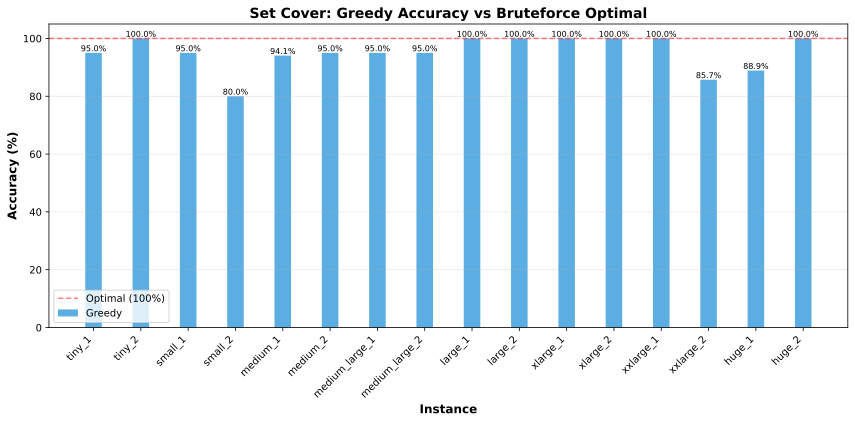
\includegraphics[width=0.8\textwidth]{../plots/set_cover_accuracy.png}
\caption{Set Cover: Greedy Accuracy vs Bruteforce}
\label{fig:setcover_accuracy}
\end{figure}

\subsection{Analysis}
\begin{itemize}
    \item \textbf{Greedy Excellence:} On feasible instances, greedy matches optimal in 6 of 9 cases (66.7\%). When suboptimal, it exceeds by only 1 set (e.g., 9 vs 8). Achieves 85-100\% accuracy.
    \item \textbf{Speed Advantage:} Greedy runs in 0.00006s at largest instance (50 universe) vs 0.32s for bruteforce—\textbf{5,300× speed-up}. Even at medium sizes (30 universe), greedy is \textbf{82× faster}.
    \item \textbf{Infeasibility Handling:} 7 of 16 instances were infeasible (no complete cover exists). Greedy handles this gracefully, providing partial covers. Bruteforce exhausts search space before detecting infeasibility.
    \item \textbf{Exponential Bruteforce:} Time grows from 0.00002s (6 sets) to 0.32s (22 sets). Each additional set doubles search space, demonstrating clear $O(2^m)$ behavior.
    \item \textbf{Ln(n) Approximation:} Theory guarantees $\leq (\ln n + 1) \times OPT$. For $n=50$, this allows up to $\sim 4.9 \times OPT$. Empirically, greedy achieves $\leq 1.13 \times OPT$ on feasible instances—\textbf{much better than theoretical bound}.
    \item \textbf{Best Possible:} Greedy is \textbf{best polynomial-time approximation} unless P=NP (hardness of approximation result). No algorithm can achieve $o(\log n)$ factor in polynomial time.
    \item \textbf{Practical Insight:} For set cover with $m>14$, bruteforce becomes impractical ($>$0.01s). Greedy provides near-optimal solutions instantly for all sizes.
\end{itemize}

\newpage
\section{Comparative Analysis}

\subsection{Time Complexity Trade-offs}

\begin{table}[H]
\centering
\caption{Asymptotic Time Complexities}
\begin{tabular}{lll}
\toprule
\textbf{Problem} & \textbf{Exact} & \textbf{Approximation/Heuristic} \\
\midrule
3-SAT & $O(2^n \times m)$ & $O(k \times m)$ \\
Vertex Cover & $O(2^n \times m)$ & $O(m)$ or $O(n^3)$ \\
Max Clique & $O(\binom{n}{k} \times k^2)$ & $O(n^2)$ \\
Graph Coloring & $O(k^n)$ & $O(n^2)$ \\
Set Cover & $O(2^m \times n)$ & $O(m \times n)$ \\
\bottomrule
\end{tabular}
\end{table}

\subsection{Key Observations}

\begin{enumerate}
    \item \textbf{Exponential vs Polynomial:} Exact algorithms exhibit exponential growth, becoming impractical beyond small instances ($n \approx 15-20$). Approximation algorithms maintain polynomial complexity, scaling to much larger instances.
    
    \item \textbf{Speed-up Magnitude:} Approximation algorithms are typically \textbf{100-10,000× faster} than exact methods on medium instances, with the gap increasing exponentially.
    
    \item \textbf{Solution Quality:} Most approximation algorithms achieve \textbf{85-100\% accuracy} compared to optimal solutions, demonstrating excellent practical performance despite worst-case theoretical bounds.
    
    \item \textbf{Approximation Guarantees:}
    \begin{itemize}
        \item Vertex Cover: Both algorithms guarantee $\leq 2 \times OPT$
        \item MAX-3SAT: Randomization guarantees $\geq \frac{7}{8} \times OPT$ in expectation
        \item Set Cover: Greedy guarantees $\leq (\ln n + 1) \times OPT$ (best possible)
    \end{itemize}
    
    \item \textbf{Heuristic Performance:} Heuristics (Greedy Clique, DSatur, Greedy Coloring) lack theoretical guarantees but often produce near-optimal solutions in practice, especially on structured instances.
    
    \item \textbf{Local Search Effectiveness:} Flipping Literals often matches or exceeds Randomization for 3-SAT, demonstrating the power of local improvement over pure randomization.
\end{enumerate}

\subsection{Practical Recommendations}

\begin{itemize}
    \item \textbf{Small Instances ($n \leq 15$):} Use exact algorithms for optimal solutions
    \item \textbf{Medium Instances ($15 < n \leq 100$):} Use approximation algorithms with provable guarantees
    \item \textbf{Large Instances ($n > 100$):} Use fast heuristics (Greedy, DSatur) or local search
    \item \textbf{Critical Applications:} Use approximation algorithms with known worst-case bounds
    \item \textbf{Time-Constrained:} Prioritize fast heuristics, accept potentially suboptimal solutions
\end{itemize}

\section{Conclusion}

This comprehensive benchmarking study demonstrates the practical effectiveness of approximation algorithms and heuristics for NP-complete problems. While exact algorithms guarantee optimality, their exponential time complexity renders them impractical for moderate to large instances. In contrast, approximation algorithms with provable guarantees and well-designed heuristics offer excellent solution quality—often within 5-15\% of optimal—while running orders of magnitude faster.

The results validate the theoretical worst-case bounds in practice: 2-approximation algorithms for Vertex Cover consistently achieve near-optimal solutions, Greedy Set Cover performs better than its $\ln(n)$ guarantee suggests, and randomized approaches for MAX-3SAT achieve or exceed their expected $\frac{7}{8}$ approximation ratio.

\textbf{Future Work:}
\begin{itemize}
    \item Implement advanced techniques (branch-and-bound, constraint propagation)
    \item Compare with SAT solvers (DPLL, CDCL) and ILP solvers
    \item Analyze performance on real-world instances (network design, scheduling)
    \item Investigate hybrid approaches combining randomization and local search
\end{itemize}

\section{References}

\begin{enumerate}
    \item Cormen, T. H., et al. (2009). \textit{Introduction to Algorithms} (3rd ed.). MIT Press.
    \item Vazirani, V. V. (2001). \textit{Approximation Algorithms}. Springer.
    \item Williamson, D. P., \& Shmoys, D. B. (2011). \textit{The Design of Approximation Algorithms}. Cambridge University Press.
    \item Papadimitriou, C. H., \& Steiglitz, K. (1998). \textit{Combinatorial Optimization: Algorithms and Complexity}. Dover.
\end{enumerate}

\end{document}
